\documentclass{article}
\usepackage{setspace}
\usepackage[explicit]{titlesec}
\usepackage{forest}
\usepackage{hyperref}
\usepackage{graphicx}
\usepackage{listings}
\usepackage{color}
\definecolor{folderbg}{RGB}{124,166,198}
\definecolor{folderborder}{RGB}{110,144,169}

\def\Size{4pt}
% Drawing for folder directories across app
\tikzset{
  folder/.pic={
    \filldraw[draw=folderborder,top color=folderbg!50,bottom color=folderbg]
      (-1.05*\Size,0.2\Size+5pt) rectangle ++(.75*\Size,-0.2\Size-5pt);
    \filldraw[draw=folderborder,top color=folderbg!50,bottom color=folderbg]
      (-1.15*\Size,-\Size) rectangle (1.15*\Size,\Size);
  }
}
\definecolor{lightgray}{rgb}{.9,.9,.9}
\definecolor{darkgray}{rgb}{.4,.4,.4}
\definecolor{purple}{rgb}{0.65, 0.12, 0.82}
\definecolor{black}{rgb}{0, 0, 0}

\lstdefinelanguage{JavaScript}{
  keywords={typeof, new, true, false, catch, function, return, null, catch, switch, var, if, in, while, do, else, case, break},
  keywordstyle=\color{blue}\bfseries,
  ndkeywords={class, export, boolean, throw, implements, import, this},
  ndkeywordstyle=\color{darkgray}\bfseries,
  identifierstyle=\color{black},
  sensitive=false,
  comment=[l]{//},
  morecomment=[s]{/*}{*/},
  commentstyle=\color{purple}\ttfamily,
  stringstyle=\color{red}\ttfamily,
  morestring=[b]',
  morestring=[b]"
}

\lstset{
   language=JavaScript,
   backgroundcolor=\color{lightgray},
   extendedchars=true,
   basicstyle=\footnotesize\ttfamily,
   showstringspaces=false,
   showspaces=false,
   numbers=left,
   numberstyle=\footnotesize,
   numbersep=9pt,
   tabsize=2,
   breaklines=true,
   showtabs=false,
   captionpos=b
}


\title{Angular - The Full Gamut}
\author{Charlie Greenman}
\renewcommand{\familydefault}{\sfdefault}
\begin{document}

\setstretch{1.5}
\tableofcontents
\maketitle{}
\section{Introduction}

The current landscape of UI development is in a very interesting place, for many
reasons. For starters, the mere capacity of web to do many tasks previously
unavailable(Add examples here), is growing by the year. In addition, frameworks
which allow for scalability, DRY development, and consistency is ever going. In
your average web application, it generally includes type checking, unit testing,
integration testing, as well as state management, and observables/effects. These
are all things that 3 years ago were not common place in the enterprise, and it
is only becoming a greater landscape as time goes on.

Angular in my opinion, having worked with other frameworks such as Elm, Vue,
React, and Cycle, is in a very unique place. I will admit, there are many
reasons as to why other to use other front end frameworks(, or if you prefer to
not call them frameworks, I understand that as well). For instance, Vue, is very
simple to use. React, is always on the cusp of cutting edge. Reason in
particular as of this writing is simply incredible. Cycle, in it's approach
towards functional programming, is refreshing. However, Angular specializes in
consistency, therefore productivity, as well as safety.

It does not surprise me that the most robust command line, by a long shot, is
with Angular. Everything, from how to style a component, folder structure,
routing, observables, state management, type checking, is agreed upon by the
entire Angular community. It is a very safe bet when building out an enterprise
application. It makes architectural decisions very easy, and it does have the
ability to layer on newer technologies, if need be, albeit harder than some
frameworks such as React. It does not surprise me, that the first full gamet
book will be written on Angular. It towers over the rest in consistency, and
that deserves a head nod.

The issue with many technical books, is that as a reader I will walk away from
it feeling like I scratched the surface. That is, I am not confident I have
covered the full gamut of that topic. So that if I plan on building it myself,
I still have to do research on my own. In addition, when I do plan on building
an app, I do not have an example app to work against. Essentially making the
book useless. Like seriously, it has me wondering the benefit of many of the
technical books I've reading lately!

As of now, it pretty much helps as discovery, and for maintaining new material.
However, learning it does not help. This book on the other hand will help you,
really one of the first of it's kind and sort of revolutionary. By offering a
QR code, with the latest commit, linked to a stackblitz, you will simaltaneously
be able to follow along while reading the book, seamlessly. In addition, when
you have read the entire book, and need to reference bits here, and there,
you can look at a specific commit for a certain part of the book, and remind
yourself how to do it once again.

In this the full gamut series, we will build a sample application. The
application will be a pixel illustrator. The ability to draw a pixel on an
artboard, and plot the coordinates on the left side. In addition, the ability to
change colors on the right side.

The intent of the book, is that it will be built in the most cuting edge
capacity. The reader should be walking away knowing, that what they have learnt
from this book is best practices, as well the Full Gamut of Angular. Being
confident, that they are aware of the full scope of the Angular ecosystem at
this time.

In addition, conventions will be casually sprinkled from time to time.
Conventions are on wide spectrum of impact. Some conventions beckon being
chosen, while others are chosen without the thought of doing so. From an
architectural perspective, they are equally as important, because choosing them
ahead of time, will save days of unneccesary re-factoring. This book as a result
will also consider conventions as part of it's architecture, and will put them
in a blue box.

In addition, this book acknowledges that there are three parts to learning:
\begin{enumerate}
  \item Discovery
  \item Maintaining
  \item Learning
\end{enumerate}

Some parts of this book are discovery, and some parts are learning. This are
parts that every book has, but this one would like to also add maintenance to
the mix. As we build out our app throughout this book, we will also repeat steps
when possible, that we have already learnt.

Part of the value of this book as well, is if this is something that you would
like to implement, the time can be minimized by using the content mentioned
in this book.

In addition, for the core part of this book. I tried, to make the core
documenation as similar to that, that can me found in the documenation, to make
it as least confusing as possible for the reader.

Some might consider this book opinion. However, after working at 5 different
companies, I can say with confidence that they all could have used the same
architecture, and component library. That is, if you a web application, that
is data heavy, trying to allow user to interact with said data, creating,
removing, updating, and deleting, this architecture will work for you. It is
therefore my opinion that this is the singular best architecture for Angular,
and I feel 100\% comfortable calling it the Definitive Guide.

Also, the idea of a good architecture, isn't neccesarily so that it goes through
everything. The idea of good architecture, is so that if something new comes up,
you will be able to have to drastically change your codebase.

This book is going to be app agnostic. However, it is going to work against the
app in order to show how technology should be integrated in real time. In
addition, there is going to be commits made in the repo alongside the book,
so that it can give a better idea of how this architecture will work in real
time.

Each section is meant to be looked through throughly before one goes ahead and
one actually does actual wokr on them. For instance, for the section on state,
it goes through the architecture for all sections on the ngrx/store. Only once
it does so, will it go through the folder/file architecture for state.


\chapter{ Building our Application }

In order to go through the full gamut of Angular, we are going to focus on as
lightweight of an application as possible. In order to go through entire Angular
architecture, we obviously do not want to over due it, nor do too little. It
goes without saying, that your classic todo app, will not suffice. Instead the
following is the application that we will be building.

We are going to call it a pixel to coordinate illustrator. The idea behind the
app, is that we should have a canvas, paint a pixel on that canvas. We then have
a coordinate, that will appear based on where pixels are currently located.

In our application we have:
\begin{enumerate}
  \item Form
    \begin{enumerate}
      \item Pixel Size
      \item Number of Rows
      \item Number of Columns
    \end{enumerate}
  \item Color Picker
    \begin{enumerate}
      \item Background Color Picker
      \item Pixel Color Picker
    \end{enumerate}
  \item Pixel Canvas
    \begin{enumerate}
      \item Pixel Grid
      \item Ability to Remove Pixel
      \item Ability to Add Pixel
      \item Ability to Change Pixel Color
    \end{enumerate}
  \item Coordinate Viewer
    \begin{enumerate}
      \item Show x Coordinate
      \item Show y Coordinate
      \item Show Pixel Size
      \item Show Pixel Color
    \end{enumerate}
\end{enumerate}

Application will be made responsive. Without further ado, let's begin our
applcation.

\maketitle{}
\section{ Angular CLI }

In any Angular setting the Angular CLI(Command Line Interface) is going to be
a good friend. The following are things which you are able to do, in the Angular
CLI:

\begin{enumerate}
  \item Create an application out of the box
  \item Generate a module
  \item Generate a component
  \item Generate a route
  \item Generate a service
  \item Serve application
  \item Test application
  \item Lint application
\end{enumerate}

\maketitle{}
\section{Introducing Nrwl Nx}

\subsection{Arguably–The Greatest Strength of Angular}

Arguably one of the greatest strengths of the Angular(2+) ecosystem is
consistency(a point we've discussed before). As a result, Angular has the most
advanced Front End Framework CLI.

\subsection{Angular CLI Shortcoming with Regards to State Management}

However, the Angular CLI does not deal with state management. State management
in Angular2, for the most part should be done using NGRX. State management in
it's self, however, can be unwieldy. For every new reducer, a new constant file,
as well as action, effect, and proper unit testing files are needed.
In addition, the Angular Framework is not built around state management. It is
easy for it to fall through the cracks, and for an app to be done without it in
the first place. Introducing the Nrwl nx CLI.

\subsection{NX CLI}
NX is built by a team called Nrwl. They are perhaps thought leaders in the
Angular space, as they well should be, being that a large part of them came
from the core Angular team. They decided to build a cli around state management.
However, using their cli comes the following pre-conditions, include the NX
Workspace.

\subsection{Introducing the NX Workspace}
One of the things that the Nrwk team really tries to push, that isn't mainstream
yet, is the concept of a workspace. Perhaps you will remember an article
floating around a while back, about
\href{https://cacm.acm.org/magazines/2016/7/204032-why-google-stores-billions-of-lines-of-code-in-a-single-repository/fulltext}
{Google's Mono Repo}. [Worth noting, this idea
has been popularized at
\href{https://code.facebook.com/posts/218678814984400/scaling-mercurial-at-facebook/}{Facebook}
as well]. The idea is that there is a singular repository for everything.
The benefits of such are
(\href{https://nrwl.io/nx/why-a-workspace}{Taken from Nrwl site}):

\begin{enumerate}
  \item Unified versioning
    \begin{enumerate}
      \item Everything at that current commit works together
      \item A label or branch can capture the same
    \end{enumerate}
  \item Promotes code sharing and reuse
    \begin{enumerate}
      \item Easy to split code into lib modules
      \item Easy to consume implement that code and the latest changes to it
    \end{enumerate}
  \item Easier dependency management
    \begin{enumerate}
      \item One node\_modules for all code
      \item One build setup (like the AngularCLI)
    \end{enumerate}
  \item Refactoring benefits
    \begin{enumerate}
      \item Code editors and IDEs are "workspace" aware
      \item Can have a single commit for a refactor that spans applications in the domain
    \end{enumerate}
  \item Consistent developer experience
    \begin{enumerate}
      \item Ensures all necessary dependent code is available
    \end{enumerate}
\end{enumerate}

Some of the biggest disadvantages include:
\begin{enumerate}
  \item Taking time to limit access to part of workspace.
  \item One upgrade in a lib, changes all areas.
  \item Make it overkill to work on a small feature.
\end{enumerate}

\maketitle{}
\section{ Using Angular CLI in an Nx Workspace }

Now that we have created an nx workspace, let's create our app. Run
\begin{verbatim}
  ng g app angularPixelIllustrator --routing
\end{verbatim}

This will create an app called angular-pixel-illustrator\footnote{that's right
angular cli will automatically convert camel case to dash case} with routing
capabilities using the Angular CLI \footnote{If you will recall, we discussed
the Angular CLI folder/file directory in the Angular CLI Chapter}.

We can now serve\footnote{I.e. run on a server for development reasons} our app,
by running:
\begin{verbatim}
  ng serve
\end{verbatim} \footnote{It's important to note, that ng serve will open up
angularPixelIllustrator by default. As we begin to add more apps, it will make
more sense to specify specific app being opened.}


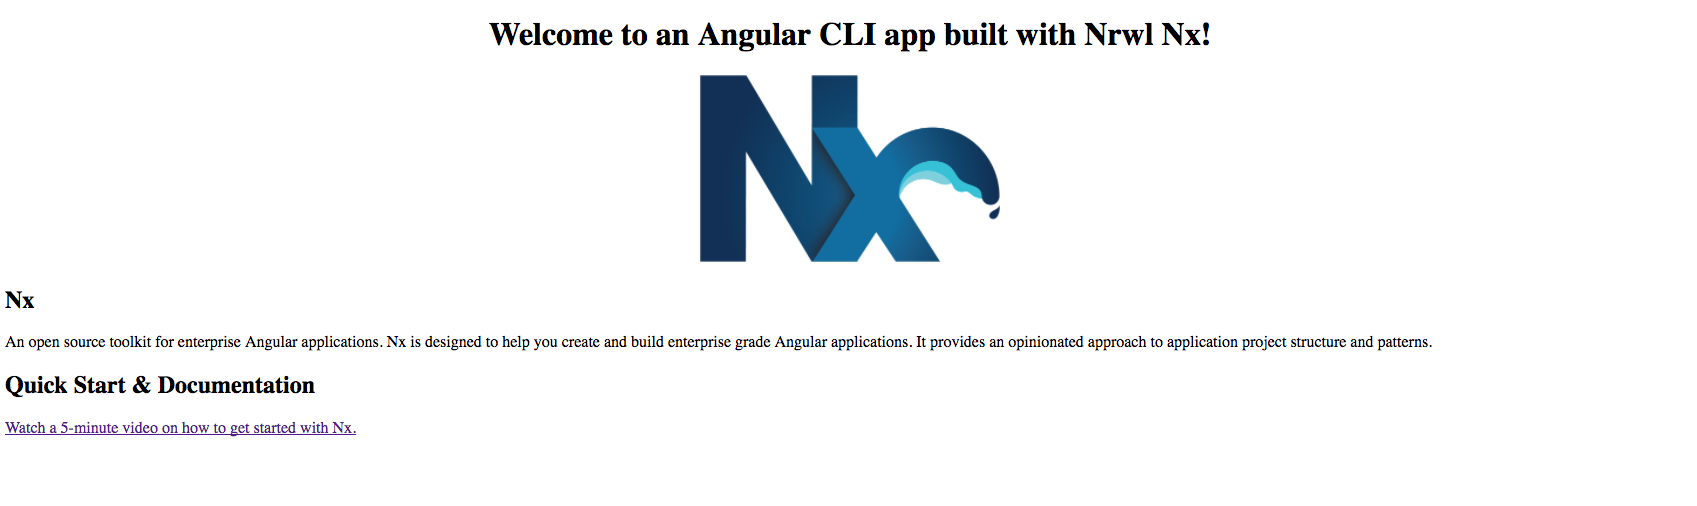
\includegraphics[width=13cm, height=9cm]{angular-cli-post-nx/angular_nx_initial_screen}

At this time, if you were to go to localhost:8080 you will see our app, is
ready to go.

Let's now create our first component. For our Pixel Illustrator, we want a form.
We will name the component chooseSize.

\subsection {Wait a Minute!}
Before we go ahead and create our component, we are going to want to tidy up
our folder architecture. The architecture we are introducing in this book is
heavily influenced by two projects. One, Nrwl, and by extension Nx. The other is
the example app, introduced in the ngrx/platform repo \footnote{It can be seen
here: https://github.com/ngrx/platform/tree/master/example-app}.

\subsubsection {Sidebar}
At the time of thiwriting there is one main area of conflict with regards to
ngrx/store v. Nx. Even though we have not experienced it yet, it makes sense to
talk about it before moving on from the cli/nx workspace chapters. Nx is very
opiniated with regards to it's folder structure. It believes everything should
be turned into it's own module, and all files related to that module should
be encapsulated inside of it. This includes (and if you are not familiar, do not
worry, we will get to it in later chaptes ) pipes, services, interfaces, guards,
and enums.

In the ngrx/example-app project, these will be split into separate folders, and
the appropriate file, will be put into that specific folder. I would imagine
that many on the ngrx/platform team agrees with nrwl/nx. I most certainly do,
and especially with state management, it makes sense for all others items to
be encapsulated into their appropiate folder. If it is something that should be
shared across app, then it should be put into it's own library. Something that
we will discuss moving forward.

\subsection {Phew, sidebar over, moving on}

The above being said, whenever we create a component, we are going to want to
encapsulate it, into a local module. That way we can add state, pipes, services,
you name it, and it will all be encapsulated in that component folder.

In order to create our module we run the following angular cli command:

\begin{verbatim}
  ng g module choose-size
\end{verbatim} \footnote{Once again we have the liberty with not having to
specify the app name}

Then, in order to create our component:
\begin{verbatim}
  ng g component choose-size
\end{verbatim}
The following five files have been created (using git diff --cached)
\begin{lstlisting}[breaklines]
new file:   apps/angular-pixel-illustrator/src/app/choose-size/choose-size.component.css
new file:   apps/angular-pixel-illustrator/src/app/choose-size/choose-size.component.html
new file:   apps/angular-pixel-illustrator/src/app/choose-size/choose-size.component.spec.ts
new file:   apps/angular-pixel-illustrator/src/app/choose-size/choose-size.component.ts
new file:   apps/angular-pixel-illustrator/src/app/choose-size/choose-size.module.ts
\end{lstlisting}

\maketitle{}
\section{ Containers, Routing + Ngrx/router }

We now have a choose-size component, as well as a choose-size module.
The dynamics of our app, is that there will only be two parent pages. One will
be the choose-size page. The other will be the draw page. When a user goes to
the page for the first time, they will see the choose-size page. Therefore we
are going to add two routes in our app.

In our app.module.ts, we will use the existing RouterModule that has been
created by Nx, and include it in our RouterModule:

\begin{verbatim}
  // Inside imports add
   RouterModule.forRoot([
    {
      path: '',
      redirectTo: 'choose-size',
      pathMatch: 'full'
    },
    {
      path: 'choose-size',
      component: ChooseSizeComponent
    }
\end{verbatim}

\marginpar{git commit -m 'Add a routes to the RouterModule, for the choose-size page.'}

Now that we have redirected the default homepage to re-direct to the
choose-size page, let's try it out. Open up http://localhost:4200, and your page
should navigate to the choose-size page, with the text, "Choose Size Works",
towards the bottom of the page. 

\maketitle{}
\section{ Mobile First - Building a Progressive Web App }

When building a an enterprise application, think about building a Progressive
Web App. It will allow your web experience to be built to feel as if it is a
native app experience. Not only will it make it progressive, but it will make
your users feel as if they are a part of an experience that is all encompassing.
It will give them the overencompassing feeling that they are getting the best
experience possible \footnote{We will discuss moving the app over to a native
app soon using NativeScript.}. Swipe right on Progressive Web Apps \footnote{
That is a millenial joke, but also a darn good PWA pun.}


\chapter{ Creating a component }

For re-iteration purposes, the definition of a component is something consituting
of a larger whole. Ideally anything we can turn into a component in an Angular
environment, will help us. In addition, anything which we can re-use across the
app, is beneficial as well.

When creating components, Angular also makes use of modules. Once again, just to
re-iterate, a module is an independent unit, which is used to construct a larger
interallated construct.

Angular stays true to these two definitions. A component can only be declared by
one component. If it is used by two, or more Angular will complain, saying that it
is already used by another component. Which by definition only constitues a larger whole.
A module on the other hand, is simply an independent unit. If we ever want to use
our component with two components, we will need to include it as part of a module.

Therefore, it is reccomended as general good practice, whenever creating a
component (unless that particular component has children), to always create it
with a module. For other reasons as well, it is smart idea. We will get into
those later \footnote{If you can't wait, and want the full list now, go here to
find it}.

We have already created a component as needed for our router, but for redundancy
sake here are the steps again.

Also, because we will be using sass, let's make sure that our cli is using sass.
Open up the .angular-cli.json file, and change two areas. One:
\begin{verbatim}
  ng set defaults.styleExt scss
\end{verbatim}
This will make it, so that whenever we set up our components using the cli,
again it will be in sass. Second, change your existing styles.css file to
styles.scss.

Let's use the cli to create our first module called choose size.
\begin{verbatim}
  ng g module choose-size
  ng g component choose-size --exports
\end{verbatim}

(The file at this time is included in our app as a route. Let's remove the
default nrwl text from app, so that all we have is choose-size works.)

\section{Architecture time}

Before, we haphazardly created a component in order to introduce routers. Now
that we are going to work on our actual component, let's set aside to specific
items with regards to architecture.

Whenever we want to create a page for our application that will be used as a
route, it is a container. Something which is simply there to "contain" all of
our components. In the root of our app directory we are going to create a
container folder. \footnote{We are once again borrowing from the example-app
project in ngrx/store}

\begin{verbatim}
  mkdir containers
\end{verbatim}
We will also be needing to mention, that we will be
moving our choose-size directory to a newly created components folder.

cd into your containers folder, and create a choose-size-page module/component:
\begin{verbatim}
  ng g module choose-size-page
  ng g component choose-size-page
\end{verbatim}

In this choose-size-page component, we will be adding our choose-size component.

In order to do so, we will need to import the choose-size component in our Angular
app, and add it to our choose-size-page module like so:

\begin{lstlisting}[caption=Importing the choose-size module]
import { ChooseSizeModule } from  '../../components/choose-size/choose-size.module';

@NgModule({
  imports: [
    CommonModule,
    ChooseSizeModule
  ],
  declarations: [ChooseSizePageComponent]
})
\end{lstlisting}

In addition, we are going to want to make sure to add an exports key/value to
our choose-size module, so that by importing it, we have the respective
component available as well.

\begin{lstlisting}[caption=Adding choose-size component as export]
  @NgModule({
   imports: [CommonModule],
   declarations: [ChooseSizeComponent],
   exports: [ChooseSizeComponent]
  })
\end{lstlisting}

With the component module properly imported, we can now use the component in our
choose-size-page html file:
\begin{verbatim}
// choose-size-page.component.html
<app-choose-size></app-choose-size>
\end{verbatim}

\maketitle{}
\section{ Adding a Route to Our Container }

At this point, being that we did not initialize our app with routing
\footnote{So that we may learn as we develop}, we will need to add a routing
file to our app. In our app root, we will be adding an app.routing.module.ts
file.

It will look something like the following:
\begin{lstlisting}[caption=app.routing.module.ts file]
import { NgModule } from '@angular/core';
import { Routes, RouterModule } from '@angular/router';

import { ChooseSizePage } from './containers/choose-size-page/choose-size-page.component';

const routes: Routes = [
  {
    path: '',
    redirectTo: 'choose-size',
    pathMatch: 'full'
  },
  {
    path: 'choose-size',
    component:  ChooseSizePage
  }
];

@NgModule({
  imports: [RouterModule.forRoot(routes)],
  exports: [RouterModule]
})
export class AppRoutingModule { }
\end{lstlisting}

In it, we are redirecting the default path to go to the choose-size url. When
the url switches over to choose-size path, it will load the choose-size component.

We are also obviously going to import the AppRoutingModule in our app.module.ts
file:
\begin{lstlisting}[caption=app.module.ts file]
import { AppRoutingModule } from './app.routing.module';
@NgModule({
  imports: [
    //...
    AppRoutingModule,
    //..
\end{lstlisting}

We are also going to delete the competing:
\begin{lstlisting}[caption=app.module.ts file]
    RouterModule.forRoot(
      [
        {
          path: '',
          redirectTo: 'choose-size',
          pathMatch: 'full'
        },
        {
          path: 'choose-size',
          component: ChooseSizeComponent
        }
      ],
      { initialNavigation: 'enabled' }
    ),
\end{lstlisting}

That we had in our app.module.ts, to tidy up that app a bit.

Terrific, we now have our app by default re-routing to the choose-size url path
and loading the choose-size component. Let's move onto styling real quick next.


\chapter{ Styling a Component }

Styling a component, of course, is a very complex topic. With styling, as an
architect in an Angular setting, there are 4 things that you will have to keep
in mind:
\begin{enumerate}
  \item Pre-processor of choice(Scss, Less, PostCss, etc.)
  \section{ Pre-processor of choice }
  \item Design system
    \begin{enumerate}
      \item Material Design(Google)
      \item Fluent Design(Microsoft)
      \item Flat Design(Apple)
    \end{enumerate}
  \item Responsive design(even if you have a mobile/tablet app)
  \item Naming convention of CSS classes
\end{enumerate}

\section{ Pre-processor of choice }
For our preprocessor, we have chosen Sass. \footnote{Incude link for a
discussion of why that is}

\section{ Naming Convention }
For our naming convention, we will go with BEM. It is an extremely easy way
of setting a part a specific component from an html and css side of things. A
quick primer on BEM.
Block is a component. We will be using pascal casing for ours \footnote{Link to
airbnb style guide}
Element is a child of block. It uses an underscore. For instance:
\begin{verbatim}
<div class = 'ChooseSize__input'></div>
\end{verbatim}
M stands for modifier. A modifier is an element, which modifies an already
existing element.
\begin{verbatim}

\end{verbatim}


\section{ Design System }
In an Angular setting, the component library which seems to make most sense is
Material Components
\footnote{https://material.angular.io/components/categories}. For starters, it
is a complete design system. All component's design will be synonymous with
each other. In addition, it is in the process of creating a cdk, which makes
all of these components customizable. In addition, it is a really nice design,
and feels native to the way Angular works. I have used it versus other libraries
and I can really say the documentation is just fantastic. I have used it in more
complex settings(e.g. the data-table), and adding on new functionality has been
just a joy.

\section{ Adding Material Design to Our App }
First install Angular Material components and Angular Animations to our app.
\begin{verbatim}
  npm install --save @angular/material @angular/cdk
  npm install --save @angular/animations
\end{verbatim}

In addition, we will need to add default styling to our app, in order for
styling to be applied to our Angular Material component. Inside of our
styles.scss file, import the following.
\begin{lstlisting}
@import '~@angular/material/prebuilt-themes/deeppurple-amber.css';
\end{lstlisting}

\section{ Our first component }
In our app, we are going to create our first component. It is essentially a form
with three fields:
\begin{itemize}
  \item Columns
  \item Rows
  \item Pixel Size
\end{itemize}

In addition, there will be a button which will say, 'Create Grid'. We are also
going to wrap our component, with the <mat-card> component, add a width of
300, margin-top and center.

\subsection{ Notable Mention - @HostBinding }
In an angular app, many times, we will want to add a specific class to our
parent container. In our situation, we will be using BEM, and creating a
ChooseSize class. It will implement flex, and use justify content, in order to
center the <mat-card> component.

\begin{lstlisting}[caption=My Javascript Example]
import { Component, HostBinding, OnInit } from '@angular/core';

@Component({
  selector: 'app-choose-size',
  templateUrl: './choose-size.component.html',
  styleUrls: ['./choose-size.component.scss']
})
export class ChooseSizeComponent implements OnInit {
  @HostBinding('class') class = 'ChooseSize';
  constructor() {}

  ngOnInit() {}
}
\end{lstlisting}

By putting @HostBinding as a decorator \footnote{If not familiar with decorator
, it is a function that is run when particular class is called} within our app,
it causes the host class to have the ChooseSize class. We are then able to
target our host element our scss:
\begin{verbatim}
  :host.ChooseSize {
    display: flex;
    justify-content: center;
  }
\end{verbatim}

\section{ CSS Naming Convention }
In your modern day front end framework, such as Angular, generally, we do not
have to worry about clashing namespaces. \footnote{Historal footnote, the
turning point for me was with this article \href{https://glenmaddern.com/articles/css-modules}{here}}.
Many other issues with css at scale, have been solved as well, have been 
solved by the general ecosystem, scss included.

However, reccomended architecture is that one still use something like BEM. I
would like to argue for using BEM in an Angular setting:
\begin{enumerate}
  \item It allows for easy grep in code base, when inspecting element first
  within chrome.
  \item It documents the type of element that it is.
  \item It will give structure to html, without need of using pug, or some other
  html pre-processor.
  \item Ease's creation of classes for integration testing\footnote{Use a modifer
  for BEM}
\end{enumerate}

It should be noted, that within our app, the form has been made a particular
width, which will work on all screen sizes, without the need of adjusting width.
As we move along in our app, we will have the option to look into sitations
wherein we can use actual media queries.

\maketitle{}
\section{ State Management - @ngrx/store }

Ngrx/store is a layer on top of Redux. It is a state management tool that was
originally created, in order to solve two way binding performance issues within
Angular. \footnote{Need to further bring source for this one}. It then extended
as a way to bring redux natively to Angular, with the use of Observables.

Let's dive into integrating @ngrx/store into our app. \marginpar{This particular
component has been written in the fashion of TDD. However, another chapter
will be dedicated to TDD/BDD in order to specify this point specifically.}

\subsection{ Using nx ngrx to Generate State }

\subsubsection{ Create root state using nx ngrx }

First we are going to generate an empty root, for our StoreModule, as well as
our EffectsModule. Our StoreModule is responsible as a singular store object,
which will be holding all of store data. Our EffectsModule is a singular effects
object, which will be holding all of our effects. \footnote{We will discuss
effects in more detail later}

\begin{lstlisting}[language=Bash]
ng generate ngrx app --module=apps/angular-pixel-illustrator/src/app/app.module.ts --onlyEmptyRoot
\end{lstlisting}

\subsubsection{ Create component state using nx ngrx }

Next, we are going to create state for our choose-size component. This is done
with ease using nx ngrx \footnote{Trust me, I've been in situations where I
was not using a CLI. It is not good news}

Run the following command:
\begin{lstlisting}[language=Bash]
ng generate ngrx choose-size --module=apps/angular-pixel-illustrator/src/app/components/choose-size/choose-size.module.ts
\end{lstlisting}

This will generate the following files:
\begin{lstlisting}[language=Bash]
create apps/angular-pixel-illustrator/src/app/components/choose-size/+state/choose-size.actions.ts (684 bytes)
create apps/angular-pixel-illustrator/src/app/components/choose-size/+state/choose-size.reducer.ts (869 bytes)
create apps/angular-pixel-illustrator/src/app/components/choose-size/+state/choose-size.effects.ts (859 bytes)
create apps/angular-pixel-illustrator/src/app/components/choose-size/+state/choose-size.effects.spec.ts (1070 bytes)
create apps/angular-pixel-illustrator/src/app/components/choose-size/+state/choose-size.reducer.spec.ts (364 bytes)
\end{lstlisting}
And update the choose-size module,
\begin{lstlisting}[language=Bash]
update apps/angular-pixel-illustrator/src/app/components/choose-size/choose-size.module.ts
\end{lstlisting}

\subsubsection{ High level overview of nx ngrx }
So, you might be wondering, what do those files that nx ngrx generated actually
do? It will generate three files:
\begin{enumerate}
  \item Action
  \item Reducer
  \item Effect
\end{enumerate}

In addition, nx will add Typescript enums for the action types. It will also
add a respective spec file(unit testing) for the action + reducer file.

\colorbox{darkgray}{\color{white}{Unit testing Actions?}}

Unit testing an action, would simply say, when an action is dispatched, expect
it to be of a certain type. However, enums, as well as type checking, fulfills
that obligation. Therefore, if one is using Typescript along with enums, there
should be no reason for writing unit tests.

\subsubsection{ Installing Redux Dev Tools }
A state environment is incomplete without proper devtools. In particular, being
able to see an action fired, as well as the complete state of any given time,
is invaluable.

Google, "redux Devtools"\footnote{In a book format, in my humble opinion, more
valuable than a link}. It is offered by remotedev.io.

With the chooseSize ngrx nx command, we just made, you should see something like
this:

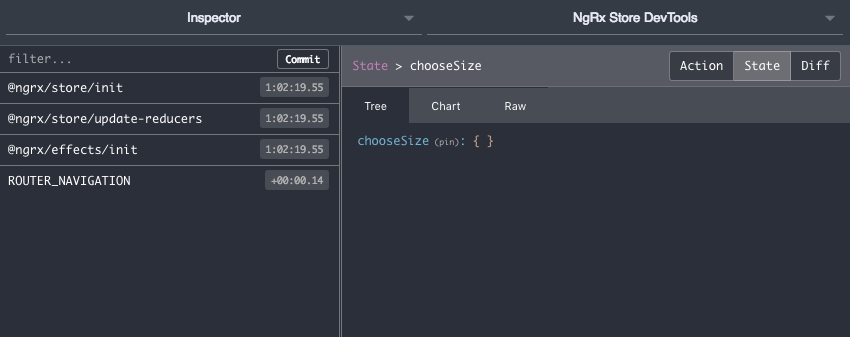
\includegraphics[width=13cm, height=9cm]{ngrx-store/redux-store}

\end{document}
